
\chapter{Grundbegriffe und \textsc{Maxwell}-Gleichungen}
\section{Kräfte und Punktladungen}

Aus der Erfahrung ergibt sich für eine ruhende Ladung

\begin{equation*}
\vec{F}(\vec{r},t)=Q\cdot\vec{E}(\vec{r},t)
\end{equation*}

Dabei ist die Ladung $Q$ eine Körpereigenschaft und $\vec{E}$ eine Eigenschaft, die die Umwelt charakterisiert. Über den Vergleich der Kraft auf zwei Körper $\vec{F}_1(\vec{r},t)=\frac{Q_1}{Q_2}\vec{F}_2(\vec{r},t)$ lässt sich so eine Einheit für die Ladung definieren.\\
\linebreak

Bei bewegten Ladungen beobachten wir etwas anderes. Die Kraft hat hier die Form

\begin{equation*}
\vec{F}=Q(\vec{E}+\vec{v}\times\vec{B})
\end{equation*}

\section{Ladungs- und Stromdichte, Ladungserhaltung}

Über eine Ladung in einem Volumenelement lässt sich der Begriff der Ladungsdichte definieren.

\begin{equation*}
\textbf{Ladungsdichte}\qquad\rho(\vec{r},t)=\diff{Q}{V}
\end{equation*}

Eine Ladungsänderung nennen wir schließlich den elektrischen Strom.

\begin{equation*}
-I:=\dot{Q}=\diff{}{t}\Int{V}{}{\rho(\vec{r},t)}{V}=\Int{V}{}{\pdiff{\rho}{t}}{V}
\end{equation*}	
Betrachten wir nun den Stromfluss durch ein Oberflächenelement d$\vec{A}$. Die Ladungsträger, welche durch diese Fläche wandern haben die Geschwindigkeit $\vec{v}$, sodass anschaulich ein kleines Volumenelement dV$ = \vec{v}\mathrm{d}t\cdot\mathrm{d}\vec{A}$ aufgespannt wird:

\begin{align*}
\mathrm{d}Q &= \rho(\vec{r},t)\vec{v}(\vec{r},t)\mathrm{d}t\mathrm{d}\vec{A}\\
\diff{Q}{t} =-I &= \rho\vec{v}\cdot\mathrm{d}\vec{A}=:\vec{j}(\vec{r},t)\cdot\mathrm{d}\vec{A}
\end{align*}

Wir nennen $\vec{j} = \rho\vec{v}$ der Anschaulichkeit nach die \textbf{Stromdichte}, denn man sieht leicht:

\begin{equation*}
\iint\limits_A\vec{j}\cdot\mathrm{d}\vec{A}=I
\end{equation*}

Setzen wir nun dies in die Gleichung für die Ladungserhaltung ein:

\begin{equation*}
0 = \dot{Q} + I = \iiint\limits_V\mathrm{d}V\pdiff{\rho}{t} \ + \oiint\limits_{\partial V}\mathrm{d}\vec{A}\cdot\vec{j} = \iiint\limits_V \mathrm{d}V\left(\pdiff{\rho}{t} + \pdiff{\vec{j}}{\vec{r}}\right) 
\end{equation*}

Da dies für für alle möglichen Volumina gelten soll, folgt daraus die

\begin{equation*}
\textbf{Kontinuitätsgleichung}\qquad\dot{\rho} + \div\vec{j} = 0
\end{equation*} 

Für den Grenzfall eines unendlich großen Volumens gilt zunächst $\vec{j}\rightarrow 0$ auf der Oberfläche, woraus man auf die für diesen Grenzfall logische Konsequenz schließen kann, dass

\begin{equation*}
\dot{Q} = -\oiint\vec{j}\mathrm{d}\vec{A} = 0
\end{equation*}

die Ladung im gesamten Raum erhalten ist.\ \\


Mit der eingeführten Stromdichte $\vec{j}$ kann man nun auch den Ausdruck der \textsc{Lorentz}kraft-Dichte $\vec{f} := \frac{\vec{F}}{V}$ definieren:

\begin{align*}
\mathrm{d}\vec{F} & = \mathrm{d}Q(\vec{E} + \vec{v}\times\vec{B}) \\
\Rightarrow \vec{f} & = \rho(\vec{r},t)\cdot(\vec{E}(\vec{r},t) + \vec{v}(\vec{r},t)\times\vec{B}(\vec{r},t) = \rho\vec{E}+ \vec{j}\times\vec{B}
\end{align*}

\section{Die \textsc{Maxwell}-Gleichungen}
Die \textsc{Maxwell}-Gleichungen wurden 1864 vom schottischen Physiker James Clerk \textsc{Maxwell} aufgestellt und bilden ein Differentialgleichungssystem für die Felder  $\vec{B}(\vec{r})$ und $\vec{E}(\vec{r})$. Zusammen mit der Kontinuitätsgleichung beschreiben sie die gesamte (klassische) Elektrodynamik, da $\rho$ und $\vec{j}$ die Quellen und Wirbel des $ \ \vec{B} \ $- und $ \ \vec{E} \ $-Feldes eindeutig bestimmen:

\begin{align*}
\div \vec{B} &= 0 \qquad\qquad\qquad\quad \epsilon_0\div \vec{E} = \rho \\
\rot \vec{E} + \dot{\vec{B}} &= 0 \qquad\qquad \frac{1}{\mu_0}\text{rot} \ \vec{B} - \epsilon_0\dot{\vec{E}} = \vec{j}
\end{align*}


Nun könnte man fragen, ob die  Beschreibung der Elektrodynamik über lokale Felder denn zweckmäßig ist oder ob man sie nicht eliminieren könnte. Das \textsc{Coulomb}-Gesetz wäre ein Beispiel für diese Fernwirkungstheorie. Zwei Gründe sprechen für die lokale Feldtheorie: sie ist zum einen schlichtweg einfacher mathematisch zu beschreiben und zum anderen unabhängig vom Vorhandensein von Materie und demzufolge Ladungsträgern.

\section{Konstruktion der \textsc{Maxwell}-Gleichungen}
Versucht man die Elektrodynamik zu beschreiben, so kann man sich zu Beginn von phänomenologischen Seite diesem Problem nähern und fordern, dass Symmetrien in Zeit und Raum die Gültigkeit der Gleichungen erhalten sollen. Dies ist eine gängige physikalische Vorgehensweise; man verlangt, dass die beschriebene (reale) Physik unabhängig von der Wahl der Koordinaten sein soll.
Wir fordern also zunächst, dass die die Form der Gleichungen unter den Symmetrietransformationen der Rauminversion $(\vec{r}\rightarrow-\vec{r})$ und der zeitlichen Reversibilität ($t\rightarrow-t$) invariant ist. Zudem wollen wir uns als Ziel setzen, die Gesetze möglichst einfach zu formulieren, das heißt, es sollen maximal Differentialgleichungen 1. Ordnung auftauchen.
Betrachten wir nun also zunächst das Transformationsverhalten verschiedener Objekte:\ \\
\ \\


\begin{tabular}{c|c|c|l}
	Objekt & $t\rightarrow-t$ & $\vec{r}\rightarrow-\vec{r}$ & Bemerkung\\
	\hline $t, \pdiff{}{t}$ & - & + & Definition\\
	$\vec{r},\pdiff{}{\vec{r}}$ & + & -& Definition\\
	$\dot{\vec{r}}$ & -& - & durch Multiplikation der Vorzeichen erhalten\\
	$\ddot{\vec{r}},\vec{F},\vec{f}$ & + & - & Erfahrung aus Mechanik:\ $\ddot{\vec{r}}=\frac{\vec{F}}{m}$\\
	$Q,\rho$ & + & + & Annahme\\
	$\vec{j}\ (=\rho\cdot\dot{\vec{r}})$ & - & - & \\
	$\vec{E}$ & + & - & Vektor, erhalten aus: $\vec{F}=Q(\vec{E}+\vec{v}\times\vec{B})$\\
	$\vec{B}$ & - & + & Pseudovektor\\
	$\pdiff{}{\vec{r}}\cdot\vec{E}$ & + & + & Skalar\\
	$\pdiff{}{\vec{r}}\cdot\vec{B}$ & - & - & Pseudoskalar\\
	$\pdiff{}{\vec{r}}\times\vec{E}$ & + & + & Pseudovektor\\
	$\pdiff{}{\vec{r}}\times\vec{B}$ & - & - & Vektor\\
	$\pdiff{}{t}\vec{E}$ & - & - & Vektor\\
	$\pdiff{}{t}\vec{B}$ & + & + & Pseudovektor
\end{tabular}
\ \\
\ \\
\ \\
\ \\
\ \\
\ \\
Da wir gefordert hatten, dass unsere gewünschten Gleichungen invariant unter den Transformationen sein sollten, dürfen wir nun nur die Größen mit dem gleichen Transformationsverhalten verknüpfen:\ \\


\begin{enumerate}
	\item
	\underline{$++$ Skalar} \quad $\rho,\div \vec{E}\\
	\\
	\Rightarrow \rho = \epsilon_0 \cdot \div\vec{E} \qquad (\epsilon_0$  ist beliebige Konstante)
	
	\item
	\underline{$--$ Vektor} \quad $\vec{j}, \rot \vec{B},\dot{\vec{B}}\\
	\\
	\Rightarrow \vec{j} = \alpha\cdot\dot{E} + \frac{1}{\mu_0}\cdot\rot \vec{B}  \qquad (\alpha,\frac{1}{\mu_0}$ sind beliebige Konstanten)
	
	\item
	\underline{$--$ Skalar} \quad $\div \vec{B}\\ 
	\\
	\Rightarrow \ 0 = \div \vec{B}$
	
	\item
	\underline{$++$ Vektor} \quad $\rot\vec{E},\dot{\vec{B}}\\
	\\
	\Rightarrow \ 0 = \rot \vec{E} + \beta\cdot\dot{\vec{B}} \qquad (\beta$  ist beliebige Konstante)
	\\
	\\
	
	\item
	\underline{$+-$ Vektor}  \quad $\vec{E},(\vec{r},\ddot{\vec{r}})\\
	\\
	\Rightarrow \ 0 =  \vec{E}$
	
	\item
	\underline{$-+$ Vektor} \quad $\vec{B}\\
	\\
	\Rightarrow \ 0 = \vec{B}$
\end{enumerate}
\ \\

Das System 1-4 ist ein widerspruchsfreies und vollständiges System von Differentialgleichungen für das $\vec{E}$- und das $\vec{B}$-Feld, da diese durch ihre Quellen und Wirbel jeweils eindeutig bis auf Konstanten bestimmt sind. Diese werden problemabhängig aus den gegebenen Randbedingungen bestimmt. Die Gleichungen 5 und 6 werden aus naheliegenden Gründen weggelassen; sie stehen zwar nicht im Widerspruch zu den ersten 4 Gleichungen, doch würde das Differentialgleichungssystem mit ihnen nur noch die Triviallösung ohne physikalisch interessante Bedeutung liefern.\
\\
\ \\
\ \\

\underline{\textbf{Konstantendiskussion:}}
\ \\
\begin{enumerate}
	\item Die Konstante $\epsilon_0$ ist zunächst frei wählbar, da die Ladung $Q$ nur bis auf einen Faktor genau bestimmt ist. Für die Wahl von $\epsilon_0$ gibt es verschiedene Ansätze:\
	\begin{enumerate}
		\item $\epsilon_0$ wird als 1 definiert. Diese Defintion wird im cgs-System umgesetzt.\
		\\
		\item $4\pi\cdot\epsilon_0$ wird 1 gesetzt. Das sich aus dieser Definition ergebende Einheitensystem nennt man das \textsc{Gauss}-System.\
	\end{enumerate}
	\ \\
	Im SI-System wird dagegen $\epsilon_0$ über $\mu_0$ festgelegt, wobei für $\mu_0$ gilt:
	
	\begin{equation*}
	[\mu_0] = \frac{[\vec{E}]}{[I]}\frac{[l]^2}{[l]}=\frac{[\vec{f}]}{[\vec{j}]}\frac{[l]}{[I]}=\frac{[\vec{F}]}{[I]^2}=\frac{N}{A^2}
	\end{equation*}
	\begin{equation*}
	\mu_0 = 4\pi\cdot 10^{-7} \frac{N}{A^2}
	\end{equation*}
	
	$\epsilon_0$ erhält man nun daraus über die Fundamentalbeziehung im SI-System:
	\begin{equation*}
	\epsilon_0\mu_0 = \frac{1}{c^2}
	\end{equation*}
	
	\item
	Die Konstante $\alpha$ erhalten wir, in dem wir von Gleichung (2) die Divergenz bilden und dann div $\vec{j}$ aus der Kontinuitätsgleichung einsetzen:
	
	\begin{equation*}
	(\epsilon_0 + \alpha) \ \pdiff{}{t} \ \div \vec{E} \overset{!}{=} 0 \; \Rightarrow \; \alpha = -\epsilon_0 
	\end{equation*}
	
	\item
	Dass die Konstante $\beta$ im SI-System gleich 1 sein musss, erhält man aus Überlegungen, dass die \textsc{Maxwell}-Gleichungen von Inertialsystem zu Inertialsystem invariant sein müssen.
\end{enumerate}
\ \\
\underline{Bemerkung:}
Im \textsc{Gauss}-System erhält man aufgrund der Wahl der Konstanten für die \textsc{Lorentz}-Kraft:
\begin{equation*}
\vec{F} = Q (\vec{E} + \frac{\vec{v}}{c}\times\vec{B})
\end{equation*}
woraus folgt:
\begin{equation*}
\epsilon_0\mu_0\cdot\beta = \frac{1}{c^2} \; \text{ und } \; \beta = \frac{1}{c}, \mu_0 = \frac{4\pi}{c}
\end{equation*}

\section{Integrale Fromulierung der \textsc{Maxwell}-Gleichungen}
Die integrale Formulierung der \textsc{Maxwell}-Gleichungen ist äquivalent zu der differentiellen und ergibt sich entweder aus Volumen- oder Flächenintegration auf beiden Seiten der entsprechenden Gleichung und dann der Anwendung der Integralsätze von \textsc{Gauss} oder \textsc{Stokes}:
\ \\
\begin{align*}
\text{i)} \quad & \epsilon_0 \ \div \vec{E} = \rho & \Leftrightarrow \qquad\qquad & \epsilon_0\oiint \mathrm{d}\vec{A} \cdot\vec{E} = Q_{\text{in}} \\
\text{ii)} \quad & \div\vec{B} = 0 & \Leftrightarrow \qquad\qquad & \oiint \mathrm{d}\vec{A}\cdot\vec{B} = 0 \\
\text{iii)} \quad & \rot \vec{E} + \dot{\vec{B}} = 0 & \Leftrightarrow \qquad\qquad & \oint\limits_{\partial A} \mathrm{d}\vec{r}\cdot\vec{E} \ + \ \iint\limits_A \mathrm{d}\vec{A}\cdot\dot{\vec{B}} = 0 \\
\text{iv)} \quad & \frac{1}{\mu_0} \ \rot \vec{B} - \epsilon_0 \dot{\vec{E}} = \vec{j} & \Leftrightarrow \qquad\qquad & \frac{1}{\mu_0}\oint\limits_{\partial A}\mathrm{d}\vec{r}\cdot\vec{B} \ - \ \epsilon_0\iint\limits_A\mathrm{d}\vec{A}\cdot\dot{\vec{E}} = I_{\text{in}}
\end{align*}
\newpage
\underline{Bemerkung:}\\

$\vec{r}$ und $t$ sind unabhängige Variablen, das heißt, dass die Felder $\vec{B}$ und $\vec{E}$ jeweils von $\vec{r}$ und $t$ abhängen, nicht aber von $\dot{\vec{r}}$.
Zudem ist es aufgrund unserer Forderungen bei der Konstruktion der \textsc{Maxwell}-Gleichungen verboten, dass eine explizite Abhängigkeit der Grundgleichungen von $\vec{r}$ und $t$ vorliegt, da es sonst außergewöhnliche Zeiten und Orte gäbe, was aber die geforderte Homogenität verletzen würde.
\section{Induktionsgesetz für Leiterschleifen}

\begin{wrapfigure}[]{l}[0cm]{0cm}
	\raisebox{0pt}[\dimexpr\height-1\baselineskip\relax]{
		\colorbox{hgrey}{
			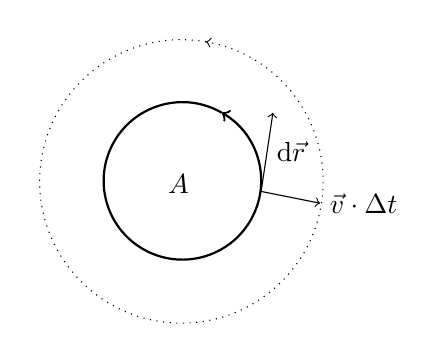
\begin{tikzpicture}
			
			\draw[thick,->] (3.2,0) arc (60:420:1);
			\draw[dotted,->] (3,0.9) arc (80:440:1.8);
			\draw[->] (3.7,-1)--node[right]{$\mathrm{d}\vec{r}$}(3.85,0) ;
			\draw[->] (3.7,-1)--(4.45,-1.15)node[right]{$\vec{v}\cdot\Delta t$} ;
			\draw (2.65,-.9) node{$A$};
			
			
			\end{tikzpicture}
		}
	}
	\caption{Flächenänderung}
\end{wrapfigure}
Zunächst definieren wir den magnetischen Fluss $\Phi$ durch eine Fläche $\vec{A}$ im Raum:

\begin{equation*}
\Phi := \iint\limits_A\mathrm{d}\vec{A}\cdot\vec{B}
\end{equation*}

Man sieht leicht, dass sich der Fluss $\Phi$ bei Flächenänderung und Änderung der magnetischen Flussdichte $\vec{B}$ ändert:\\


\begin{align*}
\Delta\Phi &=  \Delta\left(\iint\mathrm{d}\vec{A}\cdot\vec{B}\right) = \iint\limits_A\mathrm{d}\vec{A}\cdot\Delta\vec{B} \; + \; \iint\limits_{\Delta A}\mathrm{d}\vec{A}\cdot\vec{B}\\
&= \Delta t \iint\limits_A\mathrm{d}\vec{A}\cdot\pdiff{\vec{B}}{t} \; + \; \oint\limits_{\partial A}\left(\vec{v}\Delta t\times\mathrm{d}\vec{r}\right)\cdot\vec{B}\\
&= \Delta t\left(\iint\limits_A\mathrm{d}\vec{V}\cdot\dot{\vec{B}} \; - \; \oint\limits_{\partial A}\mathrm{d}\vec{r}\cdot\left(\vec{v}\times\vec{B}\right)\right)\\
\Rightarrow \dot{\Phi} &= \iint\limits_A\mathrm{d}\vec{A}\cdot\dot{\vec{B}} \; - \; \oint\limits_{\partial A}\mathrm{d}\vec{r} \ \left(\vec{v}\times\vec{B}\right)
\end{align*}

Nach Anwenden der dritten \textsc{Maxwell}-Gleichung erhält man das
\begin{equation*}\textbf{Induktionsgesetz}\qquad
U_\text{ind} =  \oint\limits_{\partial A}\mathrm{d}\vec{r} \ \left(\vec{E} + \vec{v}\times\vec{B}\right) = - \dot{\Phi}
\end{equation*}

Das letzte Minuszeichen nennt man auch die \textbf{\textsc{Lenz}`sche Regel}, welche besagt, dass ein induzierter Strom immer ein Magnetfeld erzeugt, welches seiner eigenen Ursache ($U_{\mathrm{induziert}}$) entgegengerichtet ist.
\ \\
Auffällig bei dem Induktionsgesetz ist seine Ähnlichkeit mit der auf eine freie Ladung wirkende Kraft $\vec{F} = Q(\vec{E} + \vec{v}\times\vec{B})$. Darin liegt auch die Begründung für ebenjenes Gesetz:\

Wir stellen uns eine Leiterschleife vor, welche an einer Stelle durchbrochen ist, damit kein Strom durch die Schleife fließen könnte. Auf einen sich in dieser Schleife bewegenden Ladungsträger wirkt die Kraft:

\begin{equation*}
\vec{F} = Q(\vec{E} + \vec{v}\times\vec{B}) =: Q\vec{E'}
\end{equation*} 

Man sieht, dass das $\vec{E}$-Feld abhängig vom Bezugsystem ist, daher haben wir für $\vec{E'}$ ein Bezugssystem konstruiert, welches sich mit der Geschwindigkeit $\vec{v}$ gegenüber dem Laborsystem bewegt. Damit haben wir im mitbewegeten Bezugssystem erreicht, dass $\vec{v'} = 0$ ist. Bilden wir nun das Weginteral für ein Teilchen entlang der Leiterschleife im $\vec{E}$-Feld erhalten wir:

\begin{equation*}
\oint\limits_{\mathrm{Schleife}}\mathrm{d}\vec{r}\cdot\left(\vec{E} + \vec{v}\times\vec{B}\right) = \oint\limits_{\mathrm{Schleife}}\mathrm{d}\vec{r}\cdot\vec{E'} = \int\limits_{\mathrm{Beginn}}^{\mathrm{Ende}}\mathrm{d}\vec{r}\cdot\vec{E'} = U_{\mathrm{induziert}}
\end{equation*}